\documentclass{article}

\title{Prototype Forcing File Generator}
\author{Matthew Russell}
\date{February 12 2013}


% Define stuff to use for the title page.
% copied from some french dude...
% I modified it to get it to work

\def\blurb{
  Carleton University \\
  Department of Civil and Environmental Engineering \\
  Faculty of Engineering \\[1em]
}

\def\clap#1{\hbox to 0pt{\hss #1\hss}}%

\newcommand{\cligne}[1] {
	\hbox to \hsize{
		\vbox{\centering #1}
	}
}

\newcommand{\iligne}[1] {
	\hbox to \hsize{
		\vbox{\hspace{23em} #1}
	}
}

\def\haut#1#2#3{
	\hbox to \hsize{
		\rlap{\vtop{\raggedright #1}}
		\hss
		\clap{\vtop{\centering #2}}
		\hss
		\llap{\vtop{\raggedleft #3}}
	}
}

\def\bas#1#2#3{
	\hbox to \hsize{
		\rlap{\vbox{\raggedright #1}}
		\hss
		\clap{\vbox{\centering #2}}
		\hss
		\llap{\vbox{\raggedleft #3}}
	}
}


\newcommand{\ec}{Environment Canada}
\newcommand{\saprc}{SAPRC-07A}
\newcommand{\gm}{\textsc{GEM-MACH}}
\newcommand{\ozone}{O$_3$~}
\newcommand{\no}{NO~}
\newcommand{\nox}{NO$_x$}
\newcommand{\aurams}{\textsc{AURAMS}}
\newcommand{\cmaq}{\textsc{\small{cmaq}}}
\newcommand{\spi}{\textsc{\small{spi}}}
\newcommand{\fortran}{\textsc{Fortran95}}
\newcommand{\fortrankk}{\textsc{Fortran2003}}
\newcommand{\rodas}{\emph{Rodas-3}}
\newcommand{\librmn}{\emph{librmn.a}}
\newcommand{\openmp}{OpenMP}
\newcommand{\ie}{i.e.}
\newcommand{\eg}{e.g.}

\newcommand{\code}[1]{\small{\texttt{#1}}}

% Acronyms
\usepackage[printonlyused,withpage]{acronym}
\acrodef{cmc}[CMC]{\textsc{Canadian Meteorological Centre}}
\acrodef{cam}[CAM]{\textsc{Canadian Aerosol Module}}
\acrodef{kpp}[KPP]{\textsc{Kinetic PreProcessor}}
\acrodef{nrc}[NRC]{\textsc{National Research Council}}
\acrodef{scm}[SCM]{\textsc{Source Control Management}}
\acrodef{svn}[SVN]{\textsc{Subversion}}
\acrodef{tlm}[TLM]{\textsc{Tangent Linear Model}}

% Set the margins to something like 1"
\addtolength{\hoffset}{-1cm}
\addtolength{\textwidth}{2cm}

%\addtolength{\voffset}{-1cm}
\addtolength{\textheight}{2cm}

\usepackage{minted}

% Colours...
\usepackage[pdftex]{hyperref}
\hypersetup{
    colorlinks,
    citecolor=black,
    filecolor=black,
    linkcolor=black,
    urlcolor=blue
}
\usepackage{color}

% Highlight
\usepackage{soul}

% Math stuff
\usepackage{amsthm}
\usepackage{amsmath}
\usepackage{amssymb}

% Fancy enumerate
\usepackage{enumerate}

% Ability to include other PDF documents
\usepackage{pdfpages}

\begin{document}

\maketitle

\section{Proposed Architecture}

\begin{figure}
	\centering
	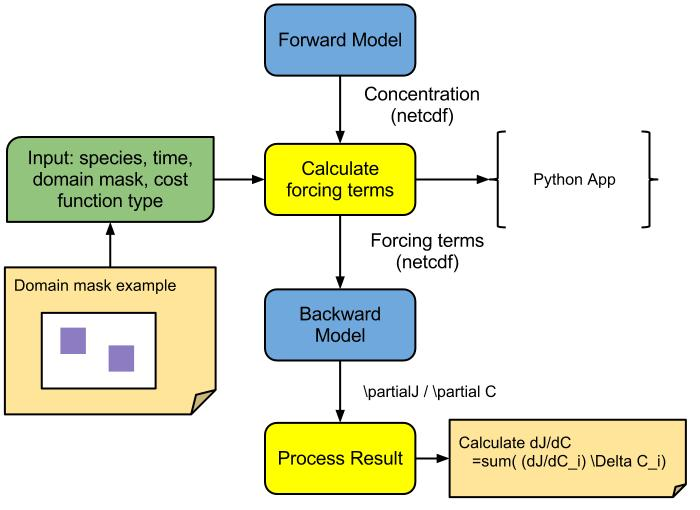
\includegraphics[width=\linewidth]{CMAQ-Adjoint-Process.jpg}
	\caption{Flowchart depicting general process flow}
	\label{process}
\end{figure}

Figure \ref{process} shows a high level process diagram for how we propose
forcing files can be generated.  This process shows that forcing files would be
generated in post processing.  This choice includes several advantages and
disadvantages.  Namely, this model limits the process to only being able to use
hour concentration output rather than concentrations at time steps only visible
during the simulation.  However, using this model, forcing term generation does
not have to be incorporated into CMAQ and as such, the tools that can be used
to implement the software are not limited to Fortran, CMAQ does not require
re-compilation for every update, and the process can be implemented in a
user-friendly graphical user interface using cross-platform compatible
software.

\section{Requirements}

Here and after, the process to generate forcing files will be referred to as ``the application''.

The application must:
\begin{itemize}
	\item be user-friendly
	\item be easy for users to incorporate their own custom forcing functions into
	\item be easily re-run for multiple simulations (i.e. settings can be saved and re-used from the command line)
	\item not be platform specific
	\item depend on software easily available
\end{itemize}

\subsection{Specification}

The application will be implemented in Python.  This choice was made as Python is a popular language in the research community, is available on virtually all platforms, very well supported, can be incorporated with Fortran (not used here, but leaves open many possibilities), easy to learn and has many online educational resources, and can be used to create graphical user interfaces.

Required packages (generally all available via package managers): python-wxglade (for wxpython), python-numpy, python-netcdf, python-dateutil.  Winder manager library is \emph{wxpython}.

\begin{itemize}
	\item Object model is such that only two classes have to be added to add a custom cost-function
	\item The application will have a ``save state'' button that can be loaded another time to re-load the settings.  This state can also be called from the command line such that this application can operate form the command line or from inside scripts.
	\item The application is broken up into four panels, one to read the simulation domain, one for general inputs that apply to all cost functions, one for the specific cost function, and one ``logging'' panel where the user receives messages about what they are setting and help messages
\end{itemize}

Processing the results of the adjoint model (the second yellow box in figure \ref{process}) will be done by a different mode in the same application.  At this time however, proposed interface designs are not yet ready to be presented.

\subsection{Proposed Application Design}

\begin{figure}
	\centering
	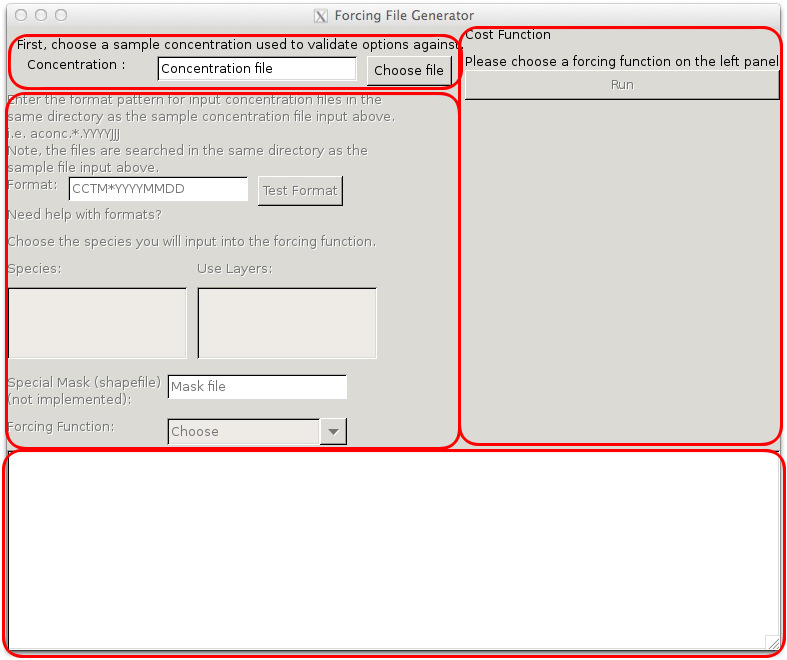
\includegraphics[width=\textwidth]{Forcing_App_Layout.jpg}
	\caption{Example of the application before any inputs are filled in.  Most inputs in this stage are disabled as the user has not yet defined the domain by providing a sample concentration file.}
	\label{ss}
\end{figure}

\begin{figure}
	\centering
	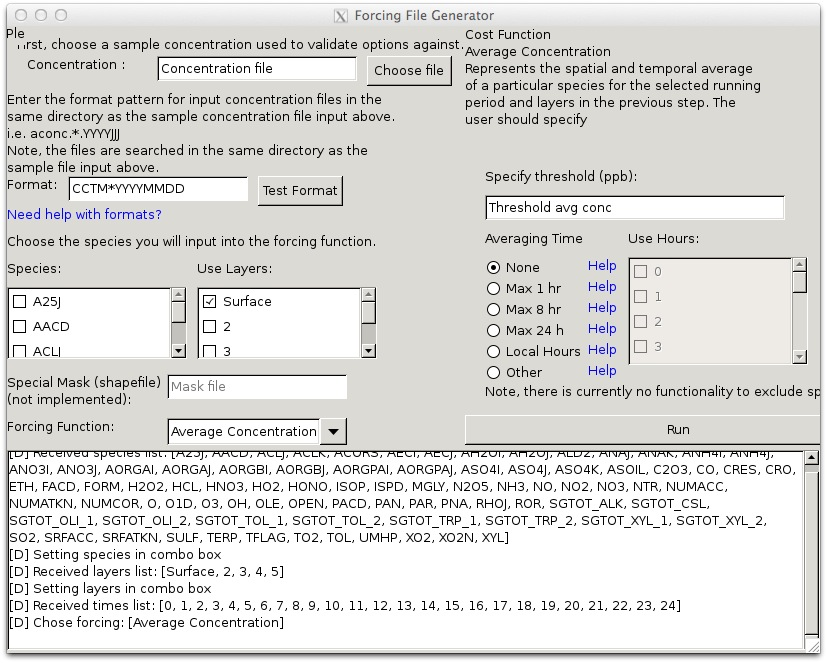
\includegraphics[width=\textwidth]{Forcing_App_Layout-filled.jpg}
	\caption{Example of the application when inputs are given and the Averaging Concentration adjoint cost function are chosen.}
	\label{ssfilled}
\end{figure}

Figures \ref{ss} and \ref{ssfilled} illustrate a preliminary design for the
application.  These figures are here to show the ease of use and potential of a
graphical user interface.  Many features in the specifications are still
missing in this proposal at this time.

\section{Science Documentation}

Figure \ref{inputs} illustrated the different inputs required for adjoint forcing field generation.

\begin{figure}
	\centering
	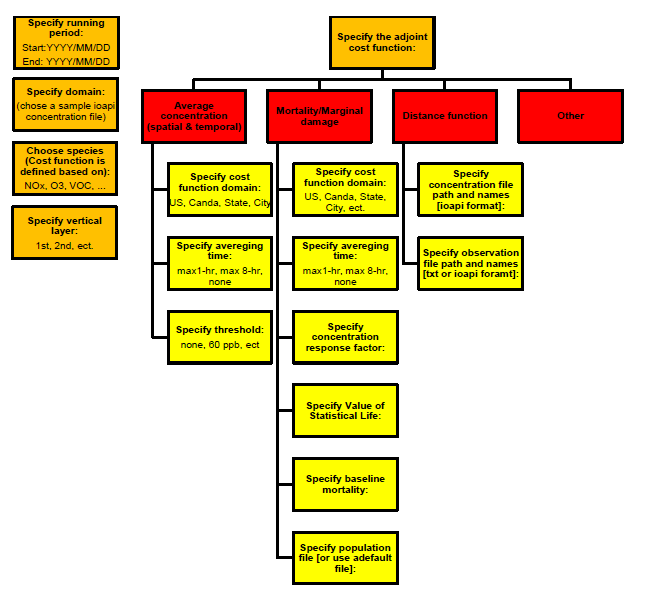
\includegraphics[width=1.2\textwidth]{Forcing-Interface-Chart.png}
	\caption{Digram illustration the different parameters required for each adjoint cost function.}
	\label{inputs}
\end{figure}


The forcing interface provides a user-friendly environment for the users to prepare forcing files for their desirable adjoint run. In this interface, the user first specifies general information before setting a specific adjoint cost function. The blue boxes denote inputs only required for the specific adjoint cost function (shown in red.)

\begin{itemize}
	\item \textbf{Running period}: which represents the beginning and end time for the run.
	\item \textbf{Simulation domain}: Domain dimensions, species, layers, time steps. These can be set in the application by pointing at a sample concentration file from the simulation
	\item \textbf{Adjoint 2D domain}: 2D Sub-domain of simulation domain to run the adjoint cost function on. This can represent a specific city, state, region, etc.
	\item \textbf{Layers}: It represents layers which the user wants to include in the adjoint cost function (this is the third dimension of the Adjoint 2D domain above). Note that for some particular applications such as mortality only the first (surface) should be selected.
	\item \textbf{Species}: The adjoint cost function is a function of the selected species.
\end{itemize}

After specifying the general information, the user can specify the cost function. Some functions are pre-defined in the interface, but the user can define any other cost function. The pre-defined functions include:

\begin{itemize}
	\item \textbf{Average concentration}: Represents the spatial and temporal average of a particular species for the selected running period and layers in the previous step. The user should specify:
	\begin{itemize}
		\item \textbf{Averaging Time}: which defines the averaging time for the concentrations used in the cost function. If none is selected, the averaging time is 24 hours.
		\item \textbf{Threshold}: which provides a flexibility for users to filter the concentrations more than the specified threshold. For example, if the user wants to see the influences of all emissions sources on grid cells where and where the concentrations violate the standard, he/she can simply set the threshold values to the standard.
	\end{itemize}
	\item \textbf{Mortality/Damage function}: which represents the number of deaths (mortality) caused by air pollution, and the corresponding health damage in dollar value (damage function). Note that if the Damage function is chosen as the adjoint cost function, the output of the adjoint model will be spatial and temporal marginal damage of emissions. Marginal damage of emissions is a known concept in environmental economics representing the influence of an additional tonne of emissions on the overall health damage. For this category the following information is required:
	\begin{itemize}
	  \item \textbf{Averaging time}: which is used because the damage functions are defined based on different averaging time.
	  \item \textbf{Concentration Response Factor}: which represents how change in concentrations is related to change in mortality, and should be entered as percentage (e.g. 0.5\%, which is equal to a response factor of 0.005). Note that this factor can be defined constant for all locations, or defined by locations. In the latter case, the user needs to provide an I/O Api file which includes the location-specific response factors.
	  \item \textbf{Value of Statistical Life}: which is defined in million dollars.
	  \item \textbf{Baseline mortality}: represents number of non-accidental deaths per a million population. The baseline mortality can also be defined by locations and users can specify an I/O Api file which includes those information.
	  \item \textbf{Population}: has a default value in the interface, but users can specify their population file in I/O Api format.
	\end{itemize}
	\item \textbf{Distance function}: is used for data assimilation to minimize the distance between the model prediction and the actual observations. In this case, the users are required to specify the concentration files as well as the observation files (in I/O Api or text format.)
	\item \textbf{User Defined}: denotes space for easily added user defined cost functions.
\end{itemize}


\clearpage
\section{Software Documentation}

Figure \ref{classdia} shows a partial UML class diagram of the structure of the application to generate adjoint forcing fields.  Missing in this diagram is the ability to save and load application state for easy use on the command line.

\begin{figure}
	\centering
	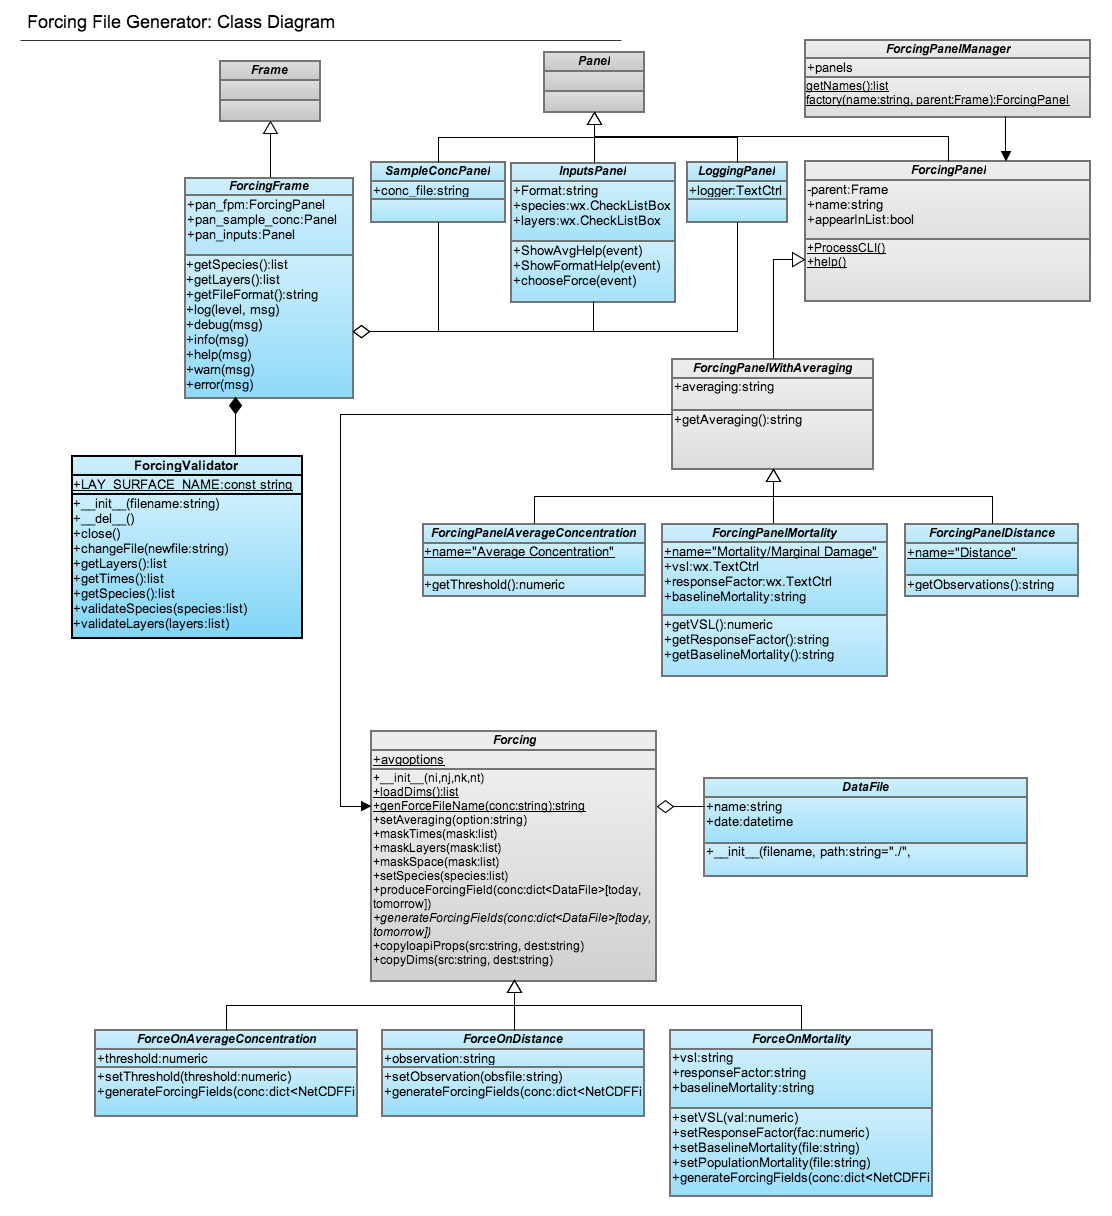
\includegraphics[width=1.2\textwidth]{Forcing_Generator.png}
	\caption{Partial class diagram of the adjoint forcing field generator.  Post results processing is not included in this diagram.}
	\label{classdia}
\end{figure}


\end{document}
